% main.tex
\documentclass{article}

\title{Feuerwerk}
\author{CoderDojo Linz}

\newcommand{\footertitle}{Feuerwerk in TypeScript}
% settings.tex
\usepackage[
    a4paper, 
    top=2cm,
    left=1cm,
    right=1cm,
    bottom=2cm
]{geometry}

\usepackage{fontspec}
\usepackage{graphicx}
\usepackage{hyperref}
\usepackage{fancyhdr}
\usepackage[ngerman]{babel}
\usepackage{wrapfig}
\usepackage{enumitem}
\usepackage{titlesec} 
\usepackage{ragged2e}
\usepackage{tcolorbox}
\usepackage{array}
\usepackage[table]{xcolor}
\usepackage{fontawesome5}

\setmainfont{Carlito}

% Fancyhdr setup
\fancypagestyle{defaultpagestyle}{
    \fancyhf{} % Clear all headers and footers
    \fancyhead[C]{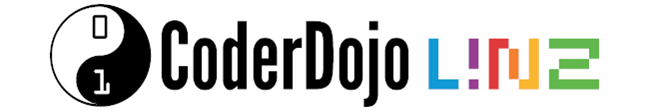
\includegraphics[width=5cm]{../../CoderDojo_Logo.png}} 
    \renewcommand{\headrulewidth}{0pt} % Remove header line
    \renewcommand{\footrulewidth}{0pt} % Remove footer line
    \fancyfoot[L]{\footertitle}
    \fancyfoot[R]{Seite \thepage} % Right footer with page number
}

\newcommand{\SectionDesign}[4]{
    \noindent
    \csname #1*\endcsname{\textcolor[HTML]{1E90FF}{\fontsize{#2pt}{#3pt}\selectfont #4}}
}

\newcommand{\TextAndImage}[5][{}]{
    \fontsize{11pt}{16pt}\selectfont
    \noindent
    \begin{minipage}[c]{#4\textwidth}
    \RaggedRight
    #2 % First parameter: text
    \end{minipage}
    \hfill
    \begin{minipage}[c]{#5\textwidth}
    \includegraphics[width=\textwidth, #1]{#3} % Second parameter: image file name
    \end{minipage}
}

\newcommand{\ImageAndText}[2]{
    \fontsize{16pt}{24pt}\selectfont
    \noindent
    \begin{minipage}[c]{0.65\textwidth}
        \includegraphics[width=\textwidth]{#1} % Second parameter: image file name
    \end{minipage}
    \hfill % Fills the space between the minipages
    \begin{minipage}[c]{0.25\textwidth}
        \centering
        #2 % First parameter: text
    \end{minipage}
}

\newcommand{\TextDesign}[1]{
    \fontsize{11pt}{16pt}\selectfont
    \noindent
    \RaggedRight
    #1 % First parameter: text
}
\graphicspath{{images/}}

\begin{document}
    \pagestyle{defaultpagestyle}

    \SectionDesign{section}{24}{24}{\textbf{Feuerwerk mit TypeScript}}
    \vspace{1cm}
     
    \ImageAndText{Feuerwerk.png}{Heute programmieren wir einen Feuerwerk-Simulator. Dabei kannst du das Tippen von Code auf der Tastatur üben und lernst Grundlagen der textuellen Programmierung kennen.
    }
    
    \vspace{2cm}
    \SectionDesign{subsection}{18}{24}{\textbf{Ziel der Übung}}
    \vspace{0.5cm}

    \TextDesign{
    Heute wollen wir gemeinsam einen Feuerwerk-Simulator programmieren. Dabei kannst du das Tippen von Code auf der Tastatur üben und lernst Grundlagen der Programmierung wie Variablen, Schleifen und Funktionen kennen.

    \vspace{\baselineskip}
    Du solltest für diese Übung schon ein wenig Programmiererfahrung mit einer Blockprogrammiersprache wie \textit{Scratch} oder \textit{Snap!} haben. Falls du noch nie Programmcode eingetippt hast, solltest du auch etwas Geduld mitbringen. Es ist am Anfang nicht immer leicht, die vielen Sonderzeichen im Code auf der Tastatur zu finden. Halte durch, Übung macht den Meister!
    }

    \vspace{1cm}
    \SectionDesign{subsection}{18}{24}{\textbf{Start}}
    \vspace{0.5cm}

    \TextDesign{
    Du brauchst für diese Übung keine spezielle Software auf deinem Computer zu installieren. Es ist nur ein aktueller Web-Browser (vorzugsweise Chrome) notwendig.
    }


    % NEWPAGE

    \newpage
    \TextDesign{
    Um loszulegen, öffne die URL \href{https://stackblitz.com/edit/feuerwerk-basics-starter?file=index.ts}{\textcolor{blue}{https://stackblitz.com/edit/feuerwerk-basics-starter?file=index.ts}}. Du wirst dadurch im Web-Browser ein Fenster sehen, das in etwa so aussieht:
    }

    \vspace{0.5cm}
    \centering
    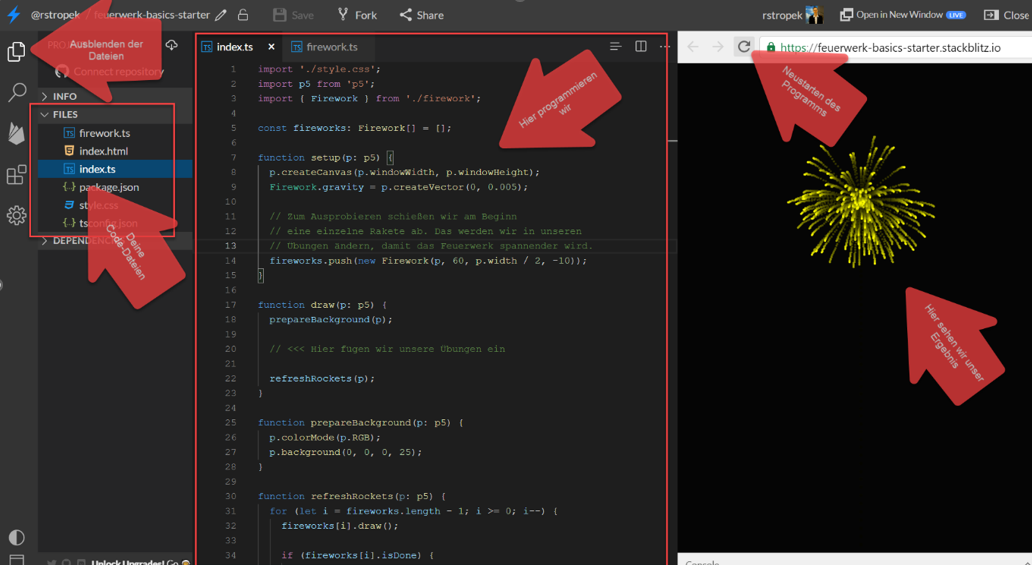
\includegraphics[width=19cm]{images/Start_Feuerwerk.png}

    \TextDesign{
        \begin{itemize}
            \item Links siehst du eine Liste der Dateien. Wir programmieren heute nur in \textit{index.ts}, daher kannst du die Dateien mit dem Symbol links oben ausblenden (siehe Pfeil Ausblenden der Dateien im Bild oben).
            \item Unseren Programmcode schreiben wir im Textfenster in der Mitte.
            \item Rechts sehen wir nach jeder Codeänderung gleich das Ergebnis.
        \end{itemize}

        In dieser Übung programmierst du mit der Programmiersprache \textit{TypeScript}. Außerdem verwenden wir die Game Engine \textit{p5js}.
    }

    \vspace{0.5cm}
    \SectionDesign{subsection}{18}{24}{\textbf{Experimente mit der ersten Rakete}}
    \vspace{0.5cm}

    \TextDesign{
    Wir haben dir unter der oben genannten URL schon ein wenig Code zum Starten vorbereitet. Ein Programm wie den Feuerwerksimulator ganz von vorne zu programmieren, ist nichts für AnfängerInnen. Dafür braucht man etwas Übung.

    \vspace{\baselineskip}
    Der von uns vorbereitete Code ist aber ziemlich dumm. Er schießt nach dem Laden der Ergebnisseite nur eine einzelne Rakete ab. Die dafür verantwortliche Zeile in unserem Code ist:

    \begin{center}
    \texttt{fireworks.push(new Firework(p, 60, p.width / 2, 75, 15));}
    \end{center}
        
    Deine Aufgabe ist, diese Codezeile zu suchen. Tipp: Sie ist in der Funktion \textit{setup}.
    }

    \vspace{0.2cm}
    \SectionDesign{subsubsection}{14}{24}{Kommentare}
    \vspace{0.2cm}

    \TextDesign{
    Die Zeilen, die mit // beginnen, sind nur Kommentare. Kommentare schreibt man in den Code, damit man später noch versteht, was man sich gedacht hat, als man den Code geschrieben hat. In diesem Fall verwenden wir Kommentare, um dir zu erklären, was die Codezeilen machen.
    }

    \vspace{0.4cm}
    \SectionDesign{subsubsection}{14}{24}{Abschießen der ersten Rakete}
    \vspace{0.2cm}

    \TextDesign{
    Hier ein paar Erklärungen zu der Codezeile zum Abschießen der Rakete:
        \begin{itemize}
            \item \textit{fireworks.push} bedeutet, dass wir eine Rakete zu einer Liste von Raketen hinzufügen, die wir auf den Bildschirm zeichnen wollen. Push ist Englisch und bedeutet \textit{schieben} oder \textit{schubsen}. Wir werden später \textit{fireworks.push} oft aufrufen, um mehr als eine Rakete zu zeichnen.
            \item \textit{new Firework} legt eine Rakete (\textit{Firework} heißt auf Deutsch \textit{Feuerwerkskörper} und \textit{new} heißt \textit{neu}) an. In den Klammern gibt man die Parameter für die Rakete an. Sie sind durch Kommas getrennt. \textbf{Achtung}: Achte beim Experimentieren darauf, dass du die Kommas nicht löschst.
        \end{itemize}
    Deine Aufgabe ist, mit den Parametern zu experimentieren. Hier ein paar Hinweise dazu:
        \begin{itemize}
            \item Den ersten Parameter \textit{p} ändere bitte nicht. Er ist aus technischen Gründen notwendig und wir gehen heute nicht näher darauf ein.
            \item Ändere den zweiten Parameter \textit{60} auf einen anderen Wert zwischen \textit{0} und \textit{360}. Hier siehst du eine Darstellung, welcher Wert zu welcher Farbe wird:

            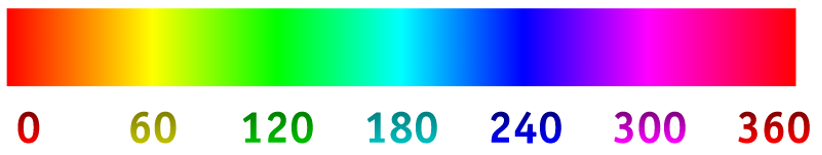
\includegraphics[width=10cm]{images/Farben.png}
            
            \item Beim dritten Parameter \textit{p.width / 2} wird die Mitte des Bildschirms errechnet. Du kannst hier statt der Formel auch eine Zahl angeben. Je kleiner die Zahl, desto weiter links erscheint die Rakete, je größer desto weiter rechts. Probiere mal 20, 200 und 400 aus. Siehst du, wie sich die Position der Rakete ändert?
            \item Der vierte Parameter 75 steuert, wie hoch die Rakete fliegen wird. 0 bedeutet, dass sie kaum abhebt und 100 bedeutet, dass sie bis zum oberen Bildschirmrand fliegen wird. Probiere mal 0, 50, 75 und 100 aus. Siehst du, wie sich die Höhe der Rakete ändert
            \item Der fünfte Parameter 15 bestimmt die Größe der Explosion. Probiere mal 10, 15 und 25 aus.
        \end{itemize}
    }

    \vspace{0.5cm}
    \SectionDesign{subsection}{18}{24}{\textbf{Mehrere Raketen}}
    \vspace{0.5cm}

    
    \SectionDesign{subsubsection}{14}{24}{Code kopieren}
    \vspace{0.2cm}

    \TextDesign{
    Statt einer Rakete möchten wir jetzt mehrere Raketen gleichzeitig abschießen. Deshalb müssen wir die Codezeile zum Abschießen der Rakete, mit der wir gerade experimentiert haben, kopieren. Weißt du schon, wie das geht?
        \begin{itemize}
            \item Stelle deinen Cursor in die Codezeile, die du kopieren möchtest.
            \item Drücke Strg + C (erst Strg, Strg gedrückt halten, dann C, danach beide Tasten loslassen), um die Zeile zu kopieren.
            \item Drücke Strg + V, um die Zeile einzufügen.
            \item Jetzt hast du die Zeile zwei Mal im Code.
            \item Deine Aufgabe ist es, die Zeile so oft zu kopieren, dass sie fünf Mal im Code ist.
        \end{itemize}
    Es macht natürlich keinen Sinn, wenn alle fünf Raketen an der gleichen Stelle losfliegen. Deine nächste Aufgabe ist es, den Code so zu ändern, dass die Raketen über die ganze Bildschirmbreite verteilt sind. So würde das aussehen:
    } 

    \begin{tcolorbox}[colback=gray!30, colframe=white]
        \begin{verbatim}
fireworks.push(new Firework(p, 60, p.width * 0 / 4, 75, 15));
fireworks.push(new Firework(p, 60, p.width * 1 / 4, 75, 15));
fireworks.push(new Firework(p, 60, p.width * 2 / 4, 75, 15));
fireworks.push(new Firework(p, 60, p.width * 3 / 4, 75, 15));
fireworks.push(new Firework(p, 60, p.width * 4 / 4, 75, 15));\end{verbatim}
    \end{tcolorbox}
    
    \SectionDesign{subsubsection}{14}{24}{Konstanten}
    \vspace{0.2cm}

    \TextDesign{
    Fällt dir auf, dass du die Farbe (60) in jeder Zeile drinnen hast? Wenn du die Farbe ändern willst, musst du fünf Mal die Zahl ändern. Das ist unpraktisch, oder? In einem solchen Fall verwendet man eine Konstante. Deine Aufgabe ist es, den Code so zu ändern, dass die Farbe nur noch einmal enthalten ist und dadurch das Ändern der Farbe einfacher wird. So muss der Code nach der Änderung aussehen:
    }

    \vspace{0.2cm}
    \begin{tcolorbox}[colback=gray!30, colframe=white]
        \texttt{\textcolor{red}{const color = 180;}} \\
        \vspace{-0.4cm}
        \begin{verbatim}
fireworks.push(new Firework(p, color, p.width * 0 / 4, 75, 15));
fireworks.push(new Firework(p, color, p.width * 1 / 4, 75, 15));
fireworks.push(new Firework(p, color, p.width * 2 / 4, 75, 15));
fireworks.push(new Firework(p, color, p.width * 3 / 4, 75, 15));
fireworks.push(new Firework(p, color, p.width * 4 / 4, 75, 15));\end{verbatim}
    \end{tcolorbox}
    \vspace{0.2cm}

    \TextDesign{
    Deine nächste Aufgabe ist, nach dem gleichen Prinzip wie bei \textit{color} auch für die Flughöhe der Raketen (vorletzter Parameter) und für die Größe der Explosion (letzter Parameter) Konstanten einzufügen und zu verwenden. So muss der Code nach der Änderung aussehen:
    }

    \vspace{0.2cm}
    \begin{tcolorbox}[colback=gray!30, colframe=white]
        \begin{verbatim}
const color = 180;\end{verbatim}
        \vspace{-0.4cm}
        \texttt{\textcolor{red}{const height = 75;}} \\
        \texttt{\textcolor{red}{const size = 15;}} \\
        \vspace{-0.4cm}
        \begin{verbatim}
fireworks.push(new Firework(p, color, p.width * 0 / 4, height, size));
fireworks.push(new Firework(p, color, p.width * 1 / 4, height, size));
fireworks.push(new Firework(p, color, p.width * 2 / 4, height, size));
fireworks.push(new Firework(p, color, p.width * 3 / 4, height, size));
fireworks.push(new Firework(p, color, p.width * 4 / 4, height, size));\end{verbatim}
    \end{tcolorbox}

    \SectionDesign{subsubsection}{14}{24}{Zufallszahlen}
    \vspace{0.2cm}

    \TextDesign{
    Immer die gleiche Farbe ist langweilig, oder? Beim Programmieren kannst du ganz einfach Zufallszahlen erzeugen. Das funktioniert ähnlich wie bei Spielen durch Würfeln. Beim Programmieren kann man aber nicht nur Zufallszahlen zwischen 1 und 6 “würfeln”, sondern beliebige Zahlen zufällig erzeugen lassen. Deine Aufgabe ist es, die Farbe zufällig vom Computer auswählen zu lassen. Du musst dafür nur den Wert der Konstanten \textit{color} wie folgt anpassen:
    }
    
    \vspace{0.2cm}
    \begin{tcolorbox}[colback=gray!30, colframe=white]
        \texttt{\textcolor{red}{const color = p.random(360);}}
    \end{tcolorbox}

    \TextDesign{
    Jedes Mal, wenn du das Programm neu startest, wird der Computer eine zufällige Farbe verwenden.
    }


    % NEWPAGE

    
    \newpage
    \SectionDesign{subsection}{18}{24}{\textbf{Raketen im Intervall abschießen}}
    \vspace{0.5cm}
    
    \SectionDesign{subsubsection}{14}{24}{Endlosschleife}
    \vspace{0.2cm}
    
    \TextDesign{
    Wir möchten unser Programm jetzt so erweitern, dass jede Sekunde Raketen abgeschossen werden. Dafür brauchen wir eine Schleife. Bei unserem ersten Experiment möchten wir fortlaufend neue Raketen abschießen. Deshalb verwenden wir eine Endlosschleife, also eine Schleife, die für immer läuft. In Scratch wäre das die Wiederhole fortlaufend-Schleife.
    }

    \TextDesign{
    Deine Aufgabe ist es, den Code so zu ändern, dass jede Sekunde Raketen starten. So muss der Code nach der Änderung aussehen:
    }

    \vspace{0.2cm}
    \begin{tcolorbox}[colback=gray!30, colframe=white]
        \texttt{\textcolor{red}{while (true) \{}} \\
        \vspace{-0.4cm}
        \begin{verbatim}
  const color = p.random(360);
  const height = 75;
  const size = 15;
  fireworks.push(new Firework(p, color, p.width * 0 / 4, height, size));
  fireworks.push(new Firework(p, color, p.width * 1 / 4, height, size));
  fireworks.push(new Firework(p, color, p.width * 2 / 4, height, size));
  fireworks.push(new Firework(p, color, p.width * 3 / 4, height, size));
  fireworks.push(new Firework(p, color, p.width * 4 / 4, height, size));\end{verbatim}
        \vspace{-0.4cm}
        \hspace{0.3cm}
        \texttt{\textcolor{red}{await delay(1000);}} \\
        \texttt{\textcolor{red}{\}}} \\
    \end{tcolorbox}

    \TextDesign{
    Die Zeile \textit{await delay(1000);} wartet 1000 Millisekunden, also eine Sekunde. Deine Aufgabe ist es, mit dieser Zahl zu experimentieren. Wie sieht das Ergebnis aus, wenn du 2000 statt 1000 verwendest? Wie beim Wert von 500?
    }
    
    \vspace{0.2cm}
    \SectionDesign{subsubsection}{14}{24}{\textit{for}-Schleife}
    \vspace{0.2cm}

    \TextDesign{
    Bereit für eine Herausforderung? Lass uns genau 10 Mal Raketen abschießen, dann soll das Feuerwerk zu Ende sein. In solchen Fällen verwendet man eine \textit{for}-Schleife. Deine Aufgabe ist es, die \textit{while}-Schleife in eine \textit{for}-Schleife umzubauen. So muss der Code nach der Änderung aussehen:
    }
    
    \vspace{0.2cm}
    \begin{tcolorbox}[colback=gray!30, colframe=white]
        \texttt{\textcolor{red}{for (let i = 0; i < 10; i++) \{}} \\
        \vspace{-0.4cm}
        \begin{verbatim}
  const color = p.random(360);
  const height = 75;
  const size = 15;
  fireworks.push(new Firework(p, color, p.width * 0 / 4, height, size));
  fireworks.push(new Firework(p, color, p.width * 1 / 4, height, size));
  fireworks.push(new Firework(p, color, p.width * 2 / 4, height, size));
  fireworks.push(new Firework(p, color, p.width * 3 / 4, height, size));
  fireworks.push(new Firework(p, color, p.width * 4 / 4, height, size));
  await delay(1000);
}\end{verbatim}
    \end{tcolorbox}

    \TextDesign{
    Hier ein paar Tipps zur \textit{for}-Schleife:

        \begin{itemize}
            \item Sie beginnt bei Null zu zählen \textit{(i = 0)}.
            \item Sie läuft solange \textit{i} kleiner als 10 ist, also zehn Mal.
            \item Bei jedem Schleifendurchlauf wird i um eins erhöht \textit{(i++)}.
        \end{itemize}
    }

    \SectionDesign{subsubsection}{14}{24}{Eine weitere \textit{for}-Schleife}
    \vspace{0.2cm}

    \TextDesign{
    Hmmm, könnten wir die \textit{for}-Schleife nicht auch verwenden, um die vielen, kopierten Aufrufe von \textit{fireworks.push} zu vereinfachen. Deine Aufgabe ist es, eine \textit{for}-Schleife zu verwenden, um aus den fünf \textit{ireworks.push}-Aufrufen einen zu machen. So muss der Code nach der Änderung aussehen:
    }
    
    \vspace{0.2cm}
    \begin{tcolorbox}[colback=gray!30, colframe=white]
        \begin{verbatim}
for (let i = 0; i < 10; i++) {
  const color = p.random(360);
  const height = 75;
  const size = 15; \end{verbatim}
        \vspace{-0.4cm}
        \hspace{0.3cm}
        \texttt{\textcolor{red}{for (let j = 0; j < 5; j++) \{}} \\
        \hspace{0.7cm}
        \texttt{\textcolor{red}{fireworks.push(new Firework(p, color, (p.width * j) / 4, height, size)); }} \\
        \hspace{0.3cm}
        \texttt{\textcolor{red}{\}}} \\
        \vspace{-0.4cm}
        \begin{verbatim}
  await delay(1000) 
} \end{verbatim}
    \end{tcolorbox}
    
    \SectionDesign{subsubsection}{14}{24}{Noch mehr Raketen...}
    \vspace{0.2cm}

    \TextDesign{
    Was müssten wir ändern, damit wir nicht nur fünf Raketen parallel abschießen können, sondern beliebig viele? Wir müssen die Obergrenzen für j anpassen und die Berechnungsformel für die X-Koordinate (horizontale Abschussposition) ändern. Das ist deine nächste Aufgabe. So muss der Code nach der Änderung aussehen:
    }
    
    \vspace{0.2cm}
    \begin{tcolorbox}[colback=gray!30, colframe=white]
        \begin{verbatim}
for (let i = 0; i < 10; i++) {
  const color = p.random(360);
  const height = 75;
  const size = 15; \end{verbatim}
        \vspace{-0.4cm}
        \hspace{0.3cm}
        \texttt{\textcolor{red}{const numberOfRockets = 10;}} \\
        \hspace{0.3cm}
        \texttt{\textcolor{red}{for (let j = 0; j < numberOfRockets; j++) \{}} \\
        \hspace{0.7cm}
        \texttt{\textcolor{red}{fireworks.push(new Firework(p, color,}} \\
        \hspace{1.5cm}
        \texttt{\textcolor{red}{(p.width * j) / (numberOfRockets - 1), height, size));}} \\
        \hspace{0.3cm}
        \texttt{\textcolor{red}{\}}} \\
        \vspace{-0.4cm}
        \begin{verbatim}
  await delay(1000);
}\end{verbatim}
    \end{tcolorbox}

    \vspace{0.2cm}
    \TextAndImage{
    Wow, da tut sich ordentlich was, oder?

    \vspace{\baselineskip}
    Hier noch ein Tipp: Wenn du ein richtig großes Feuerwerk sehen willst, das über den ganzen Bildschirm geht, klicke auf Open in \textit{New Window} (rechts oben im Bildschirmfenster), drücke danach \textit{F11} (Vollbildschirm) und zum Schluss F5 zum neu Laden. Cool, oder? Um aus der Vollbildschirmanzeige rauszukommen, drücke einfach nochmals F11.
    }{Noch_Mehr_Raketen.png}{0.4}{0.5}

    \vspace{0.5cm}
    \SectionDesign{subsection}{18}{24}{\textbf{Raketen in Formation}}
    \vspace{0.5cm}

    
    \SectionDesign{subsubsection}{14}{24}{Abwechselnde Höhe}
    \vspace{0.2cm}

    \TextDesign{
    Jetzt wollen wir unsere Raketen in Formation fliegen lassen. Damit wir vom gleichen Startpunkt ausgehen, ist deine Aufgabe, den Code zu ändern, damit er so aussieht:
    }
    
    \vspace{0.2cm}
    \begin{tcolorbox}[colback=gray!30, colframe=white]
        \begin{verbatim}
for (let i = 0; i < 100; i++) {
  const height = 75;
  const size = 15;
  const numberOfRockets = 5;
  for (let j = 0; j < numberOfRockets; j++) {
    fireworks.push(new Firework(p, p.random(360),
        (p.width * j) / (numberOfRockets - 1), height, size));
  }
  await delay(1000);
}\end{verbatim}
    \end{tcolorbox}

    \TextDesign{
    Als erstes möchten wir probieren, wie es aussieht, wenn man jede zweite Rakete nur 3⁄4 mal so hoch fliegen lässt. Hier eine Skizze, wie die Flughöhe aussehen soll:
    }

    \vspace{0.2cm}
    \centering
    \includegraphics[width=5cm]{images/Abwechselnde_Höhe.png}

    \TextDesign{
    Damit wir diese Herausforderung meistern können, brauchen wir ein wenig Mathematik. In der Schule hast du sicher schon Operationen wie Addition, Subtraktion oder Multiplikation gelernt. Es gibt beim Programmieren jedoch eine weitere Operation, die man häufig braucht: \textit{Modulo}. Modulo gibt den Rest einer Division zurück. \\
    \vspace{0.2cm}
    Hier ein paar Beispiele:
    }

    \vspace{0.25cm}
    \begin{tabular}{|l|l|l|}
        \hline
        \rowcolor{gray!30}
        Division & Ergebnis & Rest \\
        \hline
        9 / 5 & 1 & 4 \\
        \hline
        10 / 5 & 2 & 0 \\
        \hline
        5 / 2 & 2 & 1 \\
        \hline
        6 / 2 & 3 & 0 \\
        \hline
        0 / 3 & 0 & 0 \\
        \hline
    \end{tabular}
    \vspace{0.25cm}
    
    \TextDesign{
    Was hilft uns das bei unserer Herausforderung? Wenn man fortlaufende Zahlen (0, 1, 2, 3, 4, 5 etc.) modulo 2 rechnet, erhält man abwechselnd 0 und 1. Um genau zu sein erhalten wir bei geraden Zahlen die 0 als Ergebnis der Modulo-Operation und bei ungeraden 1. Hier als Tabelle dargestellt:
    }
    
    \vspace{0.25cm}
    \begin{tabular}{|l|l|}
        \hline
        \rowcolor{gray!30}
        Zahl & Ergebnis der Zahl modulo 2 \\
        \hline
        0 & 0 \\
        \hline
        1 & 1 \\
        \hline
        2 & 0 \\
        \hline
        3 & 1 \\
        \hline
        4 & 0 \\
        \hline
        5 & 1 \\
        \hline
    \end{tabular}
    \vspace{0.25cm}

    \TextDesign{
    Modulo schreibt man im Code mit dem Zeichen \%. Deine Aufgabe ist jetzt, mit diesem Wissen den geforderten Formationsflug unserer Raketen zu programmieren. So muss der Code nach der Änderung aussehen:
    }

    \begin{tcolorbox}[colback=gray!30, colframe=white]
        \begin{verbatim}
for (let i = 0; i < 100; i++) {
  const size = 15;
  const numberOfRockets = 8;
  for (let j = 0; j < numberOfRockets; j++) { \end{verbatim}
        \vspace{-0.4cm}
        \hspace{0.7cm}
        \texttt{\textcolor{red}{let height: number;}} \\
        \hspace{0.7cm}
        \texttt{\textcolor{red}{if (j \% 2 == 0) height = 90;}} \\
        \hspace{0.7cm}
        \texttt{\textcolor{red}{else height = 67.5;}} \\
        \vspace{-0.4cm}
        \begin{verbatim}
    fireworks.push(new Firework(p, p.random(360),
        (p.width * j) / (numberOfRockets - 1), height, size));
  }
  await delay(1000);
}\end{verbatim}
    \end{tcolorbox}

    \vspace{0.2cm}
    \SectionDesign{subsubsection}{14}{24}{Diagonale}
    \vspace{0.2cm}

    \TextDesign{
    Als zweite Formation möchten wir, dass die Raketen eine Diagonale bilden. Die erste Rakete soll auf Höhe 25 fliegen, die letzte auf Höhe 100. Hier eine Skizze, wie die Flughöhe aussehen soll:
    }

    \vspace{0.2cm}
    \centering
    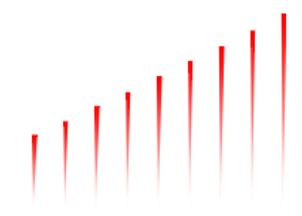
\includegraphics[width=5cm]{images/Diagonale.png}

    \TextDesign{
    Hier brauchen wir wieder etwas Mathematik. In diesem Fall hilft uns Prozentrechnung. Falls du das in der Schule noch nicht gelernt hast, ist das kein Problem. Wenn du magst, bitte eine ältere Person, eine CoderDojo-Mentorin oder einen CoderDojo-Mentor, dir das Prinzip der Prozentrechnung zu erklären. Du kannst aber auch den unten angeführten Code abtippen und Geduld haben, bis ihr Prozentrechnung in der Schule lernt.

    \vspace{\baselineskip}
    Die Höhe in unserem Fall berechnet sich wie folgt:
    \begin{itemize}
        \item Das Minimum ist 25
        \item Zu diesem Minimum addieren wir den Abstand zur Maximalhöhe \textit{(100 - 25 = 75)} multipliziert mit dem Index der Rakete \textit{j} dividiert durch die Anzahl der Raketen \textit{numberOfRockets minus 1}.
        \item Die Formel lautet also: \textit{height = 25 + 75 * j / (numberOfRockets - 1)}
    \end{itemize}

    Deine Aufgabe ist es, diese Formel in unseren Code einzubauen. So muss der Code nach der Änderung aussehen:
    }

    \begin{tcolorbox}[colback=gray!30, colframe=white]
        \begin{verbatim}
for (let i = 0; i < 100; i++) {
  const size = 15;
  const numberOfRockets = 8;
  for (let j = 0; j < numberOfRockets; j++) { \end{verbatim}
        \vspace{-0.4cm}
        \hspace{0.7cm}
        \texttt{\textcolor{red}{let height = 25 + 75 * j / (numberOfRockets - 1);}}\\
        \vspace{-0.4cm}
        \begin{verbatim}
    fireworks.push(new Firework(p, p.random(360),
        (p.width * j) / (numberOfRockets - 1), height, size));
  }

  await delay(1000);
}\end{verbatim}
    \end{tcolorbox}

    \TextDesign{
    Einen besonders schönen Effekt bekommst du, wenn du zwei Diagonalen gegenläufig erzeugst. Eine steigt von links nach rechts und die andere von rechts nach links.
    }

    \vspace{0.2cm}
    \centering
    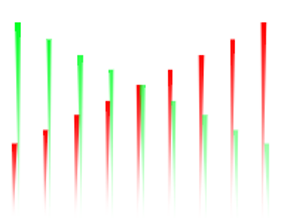
\includegraphics[width=5cm]{images/Diagonale2.png}

    \TextDesign{
    Das ist schwer theoretisch zu erklären, man muss es probieren. Deine Aufgabe ist es, den Code wie folgt zu ändern:
    }

    \begin{tcolorbox}[colback=gray!30, colframe=white]
        \begin{verbatim}
for (let i = 0; i < 100; i++) {
  const size = 15;
  const numberOfRockets = 8;
  for (let j = 0; j < numberOfRockets; j++) {
    let height = 25 + 75 * j / (numberOfRockets - 1); \end{verbatim}
        \vspace{-0.4cm}
        \hspace{0.7cm}
        \texttt{\textcolor{red}{fireworks.push(new Firework(p, 60,}} \\
        \hspace{1.5cm}
        \texttt{\textcolor{red}{(p.width * j) / (numberOfRockets - 1), height, size));}} \\
        \hspace{0.7cm}
        \texttt{\textcolor{red}{fireworks.push(new Firework(p, 120,}} \\
        \hspace{1.5cm}
        \texttt{\textcolor{red}{(p.width * j) / (numberOfRockets - 1), 25 + 100 - height, size));}} 
        \vspace{-0.4cm}
        \begin{verbatim}
  }

  await delay(3000);
}\end{verbatim}
    \end{tcolorbox}

    \vspace{0.5cm}
    \SectionDesign{subsection}{18}{24}{\textbf{Text hinzufügen}}
    \vspace{0.5cm}

    \TextDesign{
    Zum Abschluss möchten wir noch einen Glückwunsch (z. B. Neujahrswünsche, Geburtstagswünsche) zu unserem Feuerwerk hinzufügen. Das kannst du mit wenigen Zeilen Code in der \textit{draw}-Funktion erledigen. Deine letzte Aufgabe für heute ist es, die \textit{draw}-Funktion zu suchen und die folgenden Zeilen für die Textausgabe hinzuzufügen:
    }

    \begin{tcolorbox}[colback=gray!30, colframe=white]
        \begin{verbatim}
function draw(p: p5) { \end{verbatim}
        \vspace{-0.4cm}
        \hspace{0.3cm}
        \texttt{\textcolor{red}{p.colorMode(p.RGB);}} \\
        \hspace{0.3cm}
        \texttt{\textcolor{red}{p.background(0, 0, 0, 25);}} \\
        
        \vspace{\baselineskip}
        \hspace{0.3cm}
        \texttt{\textcolor{red}{p.fill('red');}} \\
        \hspace{0.3cm}
        \texttt{\textcolor{red}{p.textSize(60);}} \\
        \hspace{0.3cm}
        \texttt{\textcolor{red}{p.textStyle(p.BOLD);}} \\
        \hspace{0.3cm}
        \texttt{\textcolor{red}{p.textAlign(p.CENTER, p.CENTER);}} \\
        \hspace{0.3cm}
        \texttt{\textcolor{red}{p.text('Schönes,\textbackslash nneues Jahr\textbackslash n \faGlassCheers \faCocktail \faBirthdayCake', p.width / 2, p.height / 4);}}
        \vspace{-0.4cm}
        \begin{verbatim}
       
  // Hier folgt die for-Schleife, die wir zuvor programmiert haben
  for (let i = fireworks.length - 1; i >= 0; i--) {
    ...
  }
}\end{verbatim}
    \end{tcolorbox}
    
\end{document}
